

\section{Review of the Zebrafish Early Developmental Mechanics}

Our goal in this chapter is to identify the different phases of the developing early zebrafish embryo that our model should account for, and the different components with their characteristic scales that are expected to be at play and underlie the biomechanics of this process.

The zebrafish gastrulation, its processes and underlying causalities have long been and remain today a very active field of research. The global view that we have formed about this phenomenon, and which we present in this chapter, is based on raw microscope observations, the 3D+time imaging and reconstructions performed by the BioEmergences platform, and the state-of-the-art literature surveyed in the following publications:
\begin{itemize}
	\item D'Amico, L.A. \& Cooper, M.S., 2001. Morphogenetic domains in the yolk syncytial layer of axiating zebrafish embryos. \textit{Developmental dynamics: an official publication of the American Association of Anatomists}, 222(4), pp.611–624. \cite{DAmico:2001ic}
	\item Montero, J.-A. \& Heisenberg, C.-P., 2004. Gastrulation dynamics: cells move into focus. \textit{Trends in cell biology}, 14(11), pp.620–627. \cite{Montero:2004hh}
	\item Solnica-Krezel, L., 2005. Conserved Patterns of Cell Movements during Vertebrate Gastrulation. \textit{Current Biology}, 15(6), pp.R213–R228. \cite{SolnicaKrezel:2005uz}
	\item Solnica-Krezel, L., 2006. Gastrulation in zebrafish -- all just about adhesion? \textit{Current opinion in genetics \& development}, 16(4), pp.433–441. \cite{SolnicaKrezel:2006dl}
	\item Rohde, L.A. \& Heisenberg, C.-P., 2007. Zebrafish gastrulation: cell movements, signals, and mechanisms. \textit{International review of cytology}, 261, pp.159–192. \cite{Rohde:2007ba}
	\item Heisenberg, C.-P. \& Solnica-Krezel, L., 2008. Back and forth between cell fate specification and movement during vertebrate gastrulation. \textit{Current opinion in genetics \& development}, 18(4), pp.311–316. \cite{Heisenberg:2008fc}
	\item Chan, T.-M. et al., 2009. Developmental gene regulatory networks in the zebrafish embryo. \textit{Biochimica et biophysica acta}, 1789(4), pp.279–298.\cite{Chan:2009er}
	\item Blanchard, G.B. \& Adams, R.J., 2011. Measuring the multi-scale integration of mechanical forces during morphogenesis. \textit{Current opinion in genetics \& development}, pp.1–11.\cite{Blanchard:2011hk}
\end{itemize}

We interpret the early zebrafish embryo biomechanics to result from the interaction of the blastoderm cells isolated from the yolk cell by the 32-cell stage (or somewhat later), which first differentiate in the epithelial enveloping layer (\textit{EVL}) and the deep cells, with the \textit{deep cells} giving rise to the \textit{hypoblastic} and \textit{epiblastic} layers through gastrulation (Fig. \ref{zebrafish_10h_review_kimmel_drawings_augmented}). The epiblast is described as fated to neural and non-neural ectoderm and the hypoblast is fated to the mesoderm and the endoderm.
\begin{figure}
\begin{center}
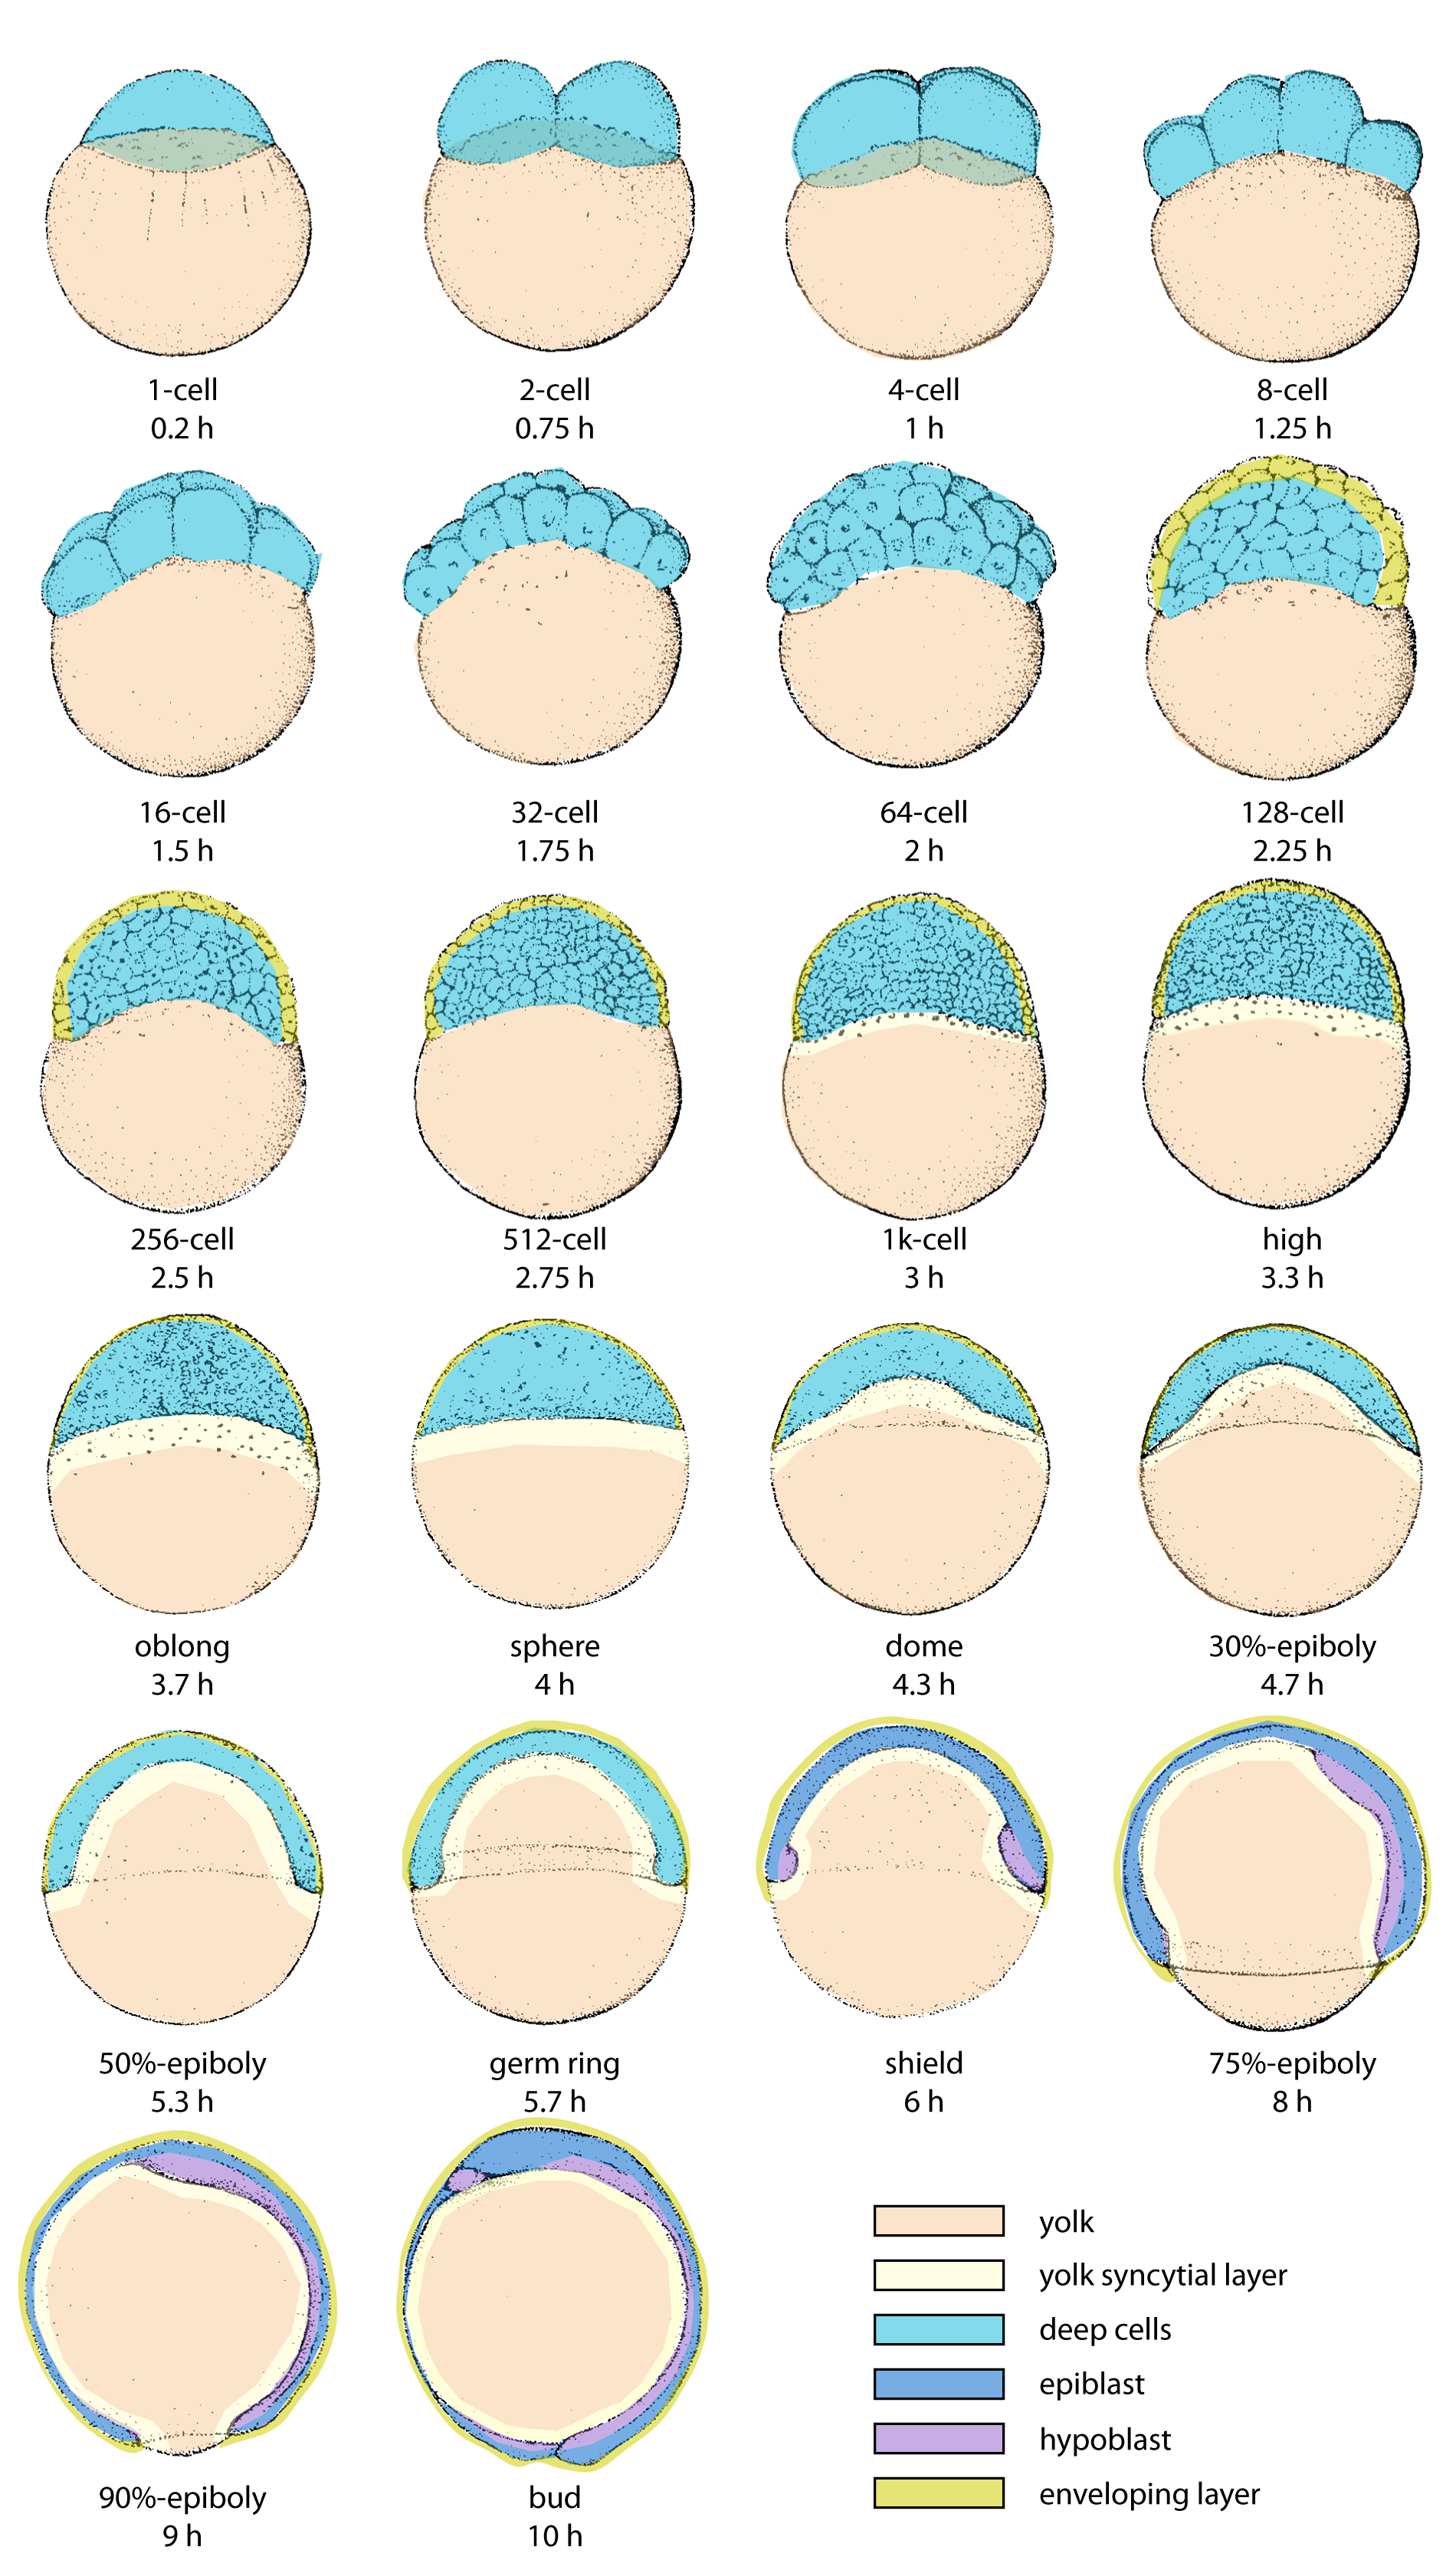
\includegraphics[width=0.6\textwidth]{../../images/zebrafish_10h_review/kimmel_drawings_augmented.png}
\end{center}
\caption{\textbf{The zebrafish early developmental stages. } Adapted from Kimmel \cite{Kimmel:1995kn}. From the 1-cell stage until the end of gastrulation, lateral views with animal pole to the top and dorsal side, identified by the shield stage, to the right. The enveloping layer (EVL) is in yellow. The deep cells (in blue) lead through gastrulation to the hypoblast (in purple) and the epiblast (in dark blue).  The whole spatio-temporal sequence is expected to last 10 hours at 28.5 degree celsius. 
%  Compléter XXXX selon instruction fichier nadine 
}
\label{zebrafish_10h_review_kimmel_drawings_augmented}
\end{figure}

Cell biomechanics is expected to result from the dynamics of the cytoskeleton. The tissue biomechanics should result from cell dynamics, including adhesive properties and intrinsic motility, cell-cell and cell-extra cellular matrix (\textit{ECM}) interactions. In addition, the yolk contribution to the embryo biomechanics during early embryonic stages is highly debated \cite{Behrndt:2012gy}.  

It is one of our main  modeling challenges to identify and integrate the components that we hypothesize to be causal in the zebrafish early embryo morphogenesis. During our more detailed exploration of the possible ingredients of the model, we will follow the known chronology of events, keeping in mind at the same time that the classical narrative of the developmental stages might also be hiding other changes in the cell dynamics. It should be one of the strengths of the model to point to the transitions in the system's dynamics.
%  ====================================================================== 


\subsection{Cleavage Stages, Formation of the EVL and YSL}
%  ====================================================================== 


We call \textit{cleavage stages} the steps going from the 1-cell stage to the 1000-cell stage through successive cell divisions. As emphasized by Olivier et al. \cite{Olivier:2010jz}, cell cycles gradually desynchronize from cell cycle 2. The first 10 cell cycles leave only time for a succession of S and M phases, and the observed lengthening is interpreted to reflect the exhaustion of maternal components required for the underlying biochemistry. Major aspects of these steps are, in addition, the absence of cell intrinsic motility, the acquisition of cell diversity in terms of cell environment and cell volume---although the global cell volume is supposed to remain constant with the sum of the daughter cells volume equal to their mother's volume without growth. The latter is actually expected to hold true until the end of gastrulation, i.e. until cycle 15 or so. Shaping the zebrafish blastoderm at these early stages is also based on cell division orientation, and precise quantitative data has been obtained providing rules of orientation from one division to the other and relative to the embryo surface \cite{Olivier:2010jz}. Two major morphogenetic events should additionally be singled out: the formation of the enveloping layer (EVL) and the formation of the yolk syncytial layer (YSL).
%  ---------------------------------------------------------------------- 


\subsubsection{The Formation of the Enveloping Cell Layer (EVL)}
%  ---------------------------------------------------------------------- 


The EVL, long considered as an extraembryonic tissue, might rather be homologous to mammals' epidermis as recently pointed by the work of D. Wagner and coll. (Communication, Madison zebrafish meeting 2012). When formed and anchored on the yolk membrane, the EVL will bring a major biomechanical constraint to the blastoderm and to the whole embryo.

EVL differentiation is described to start as early ad the 64-cell stage, and it should be a compartment by the sphere stage (4 hpf). This means that at some point inbetween these two stages, the outer layer of the blastoderm will be characterized by specific dynamics and biomechanical properties distinct from the blastoderm deep cells. Indeed, EVL is revealed as the external layer of the deep cells during the mid-blastula transition. Its cells start flattening along the radial axis and their cell cycle lengthens \cite{Kane:1992gw}.

According to Kimmel \cite{Kimmel:1985vc}, EVL cell division produces deep cells as late as the $9^{\mathrm{th}}$ cell cycle. It is shown by injections of lineage tracer dye into single blastomeres in midblastula embryos, which yield clones contributing cells to several tissues. In the example shown in Fig. 2 of \cite{Kimmel:1985vc}, "a cell of the surface enveloping layer (EVL) of the blastoderm was injected at the 1000-cell stage (3 hpf); and eventually gave rise to three classes of descendants at three separate locations: ... EVL, two adjacent somites, neural cells in the spinal cord". By the sphere stage (4 hpf), EVL cell division orientation is confined to the tangential plane of the blastoderm \cite{Kimmel:1990us}. However, mechanisms underlying the EVL differentiation are still debated \cite{Manning:2010ce}\cite{Krens:2011ht}. 
%  XXXX nadine: A toi de sortir un message de ce debat. Je n'ai pas le temps de revenir voir ces papiers. 

%  ---------------------------------------------------------------------- 


\subsubsection{The Formation of the Yolk Syncitial Layer (YSL)}
%  ---------------------------------------------------------------------- 


By cycle 9 (512-cell stage) starts the "mid-blastula transition" (MBT) and the zygotic transcription begins. At the same time, the yolk becomes a syncytium. The yolk is described at first as a large sac filled with yolk platelets and fat droplets, which are surrounded by a lipid bilayer membrane and structured by an actomyosin cortex organized soon after the egg is laid down. The yolk becomes a syncytium through one round of cell divisions at the blastoderm margin, fusing half of the mother cells' progeny with the yolk. We then distinguish the yolk syncytial layer (\textit{YSL}) where the yolk syncytial nuclei (\textit{YSN}) lie, from the yolk cytoplasmic layer (\textit{YCL}). The YSL is further divided into the internal and the external YSL. The YSL becomes an active region of transcriptional activity contributing to the dorso-ventral symmetry breaking \cite{Hong:2010ej}. The MBT certainly marks major changes in terms of the system's biomechanics. Cells acquire an intrinsic motility, the EVL differentiates and the yolk syncytium cytoskeleton further organizes.
%  ====================================================================== 


\subsection{Blastula Stages and the Onset of Epiboly}
%  ====================================================================== 


The causes of the blastoderm shape changes after MBT (3 hpf) for the next hour, i.e. until the sphere stage and the first manifestations of epiboly, remain elusive. The qualitative description highlighted by the actual naming of the developmental stages: "high", "oblong", and "sphere", points to the flattening of the blastoderm and suggests that the overall shape of the embryo gets closer to perfectly spherical. An increase of cell-cell tension compared to yolk-cell tension might lead to the flattening of the blastoderm. Other issues might include the EVL differentiation and modification of the yolk cytoskeleton organization and dynamics.

By the sphere stage (4 hpf at 28.5 degree Celsius), the YSL and YCL are well organized with dense networks of microtubules \cite{Kimmel:1985uh}\cite{SolnicaKrezel:2002ty}. Two different microtubule networks are found in the yolk: one in the anuclear yolk cortical layer, which is oriented along the animal-vegetal axis toward the vegetal pole; the other in the yolk syncytial layer, linking YSN mitotic and interphase microtubules. No microtubules were detected in the deeper, yolk-containing center of the yolk cell, but it might be an experimental artifact \cite{SolnicaKrezel:1994wl} (Fig. \ref{zebrafish_10h_review_krezel_1994}).
\begin{figure}
\begin{center}
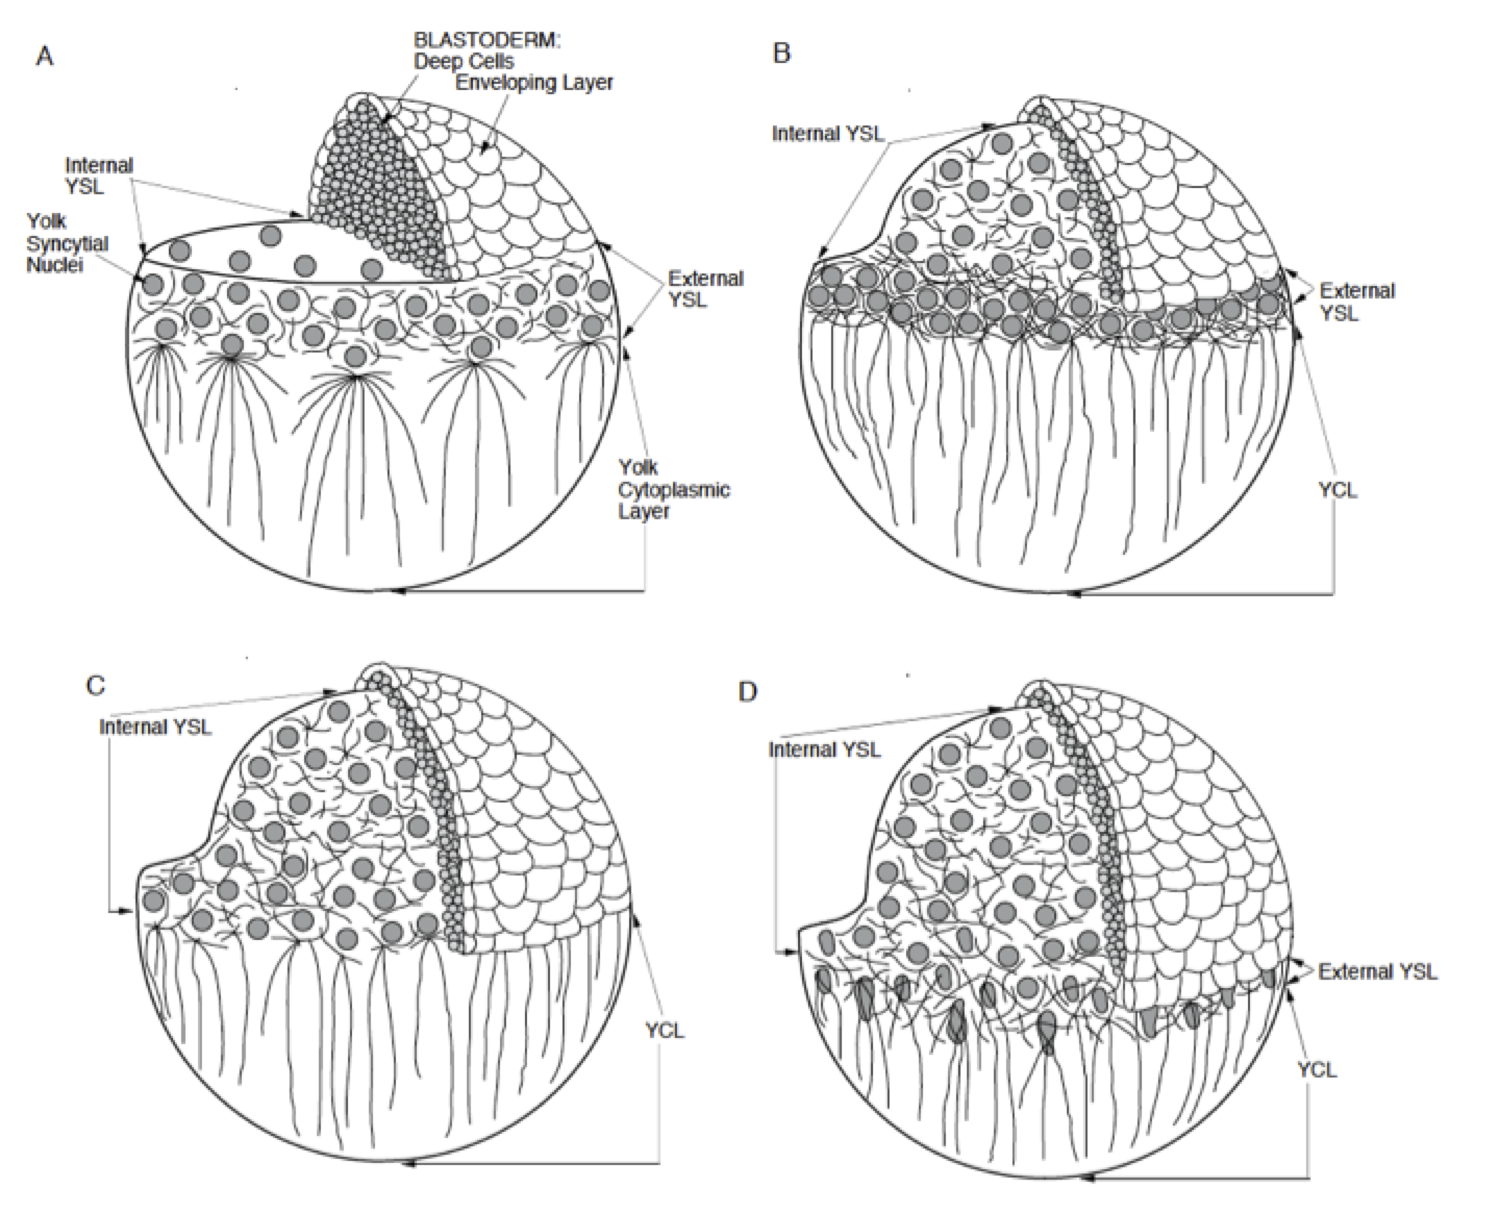
\includegraphics[width=0.6\textwidth]{../../images/zebrafish_10h_review/krezel_1994.png}
\end{center}
\caption{\textbf{Schematic illustration of the changes in the organization of the cortical cytoplasm of the yolk cell in relation to other cell types in zebrafish embryo during epiboly in normal embryos.} The organization of microtubule networks in the YSL and YCL observed in this study is indicated by thin lines. Only part of the blastoderm is shown to reveal the morphology of the yolk cell. The relative sizes of elements are not proportional. (A) The late blastula just before the onset of epiboly (sphere stage, 4.0 h). The blastoderm, composed of the internal deep cells and the superficial enveloping layer (EVL), is positioned atop of the syncytial yolk cell. The animal surface of the yolk cell underlying the blastoderm is flat. Most of the yolk syncytial nuclei (YSN) are in the external yolk syncytial layer (external YSL) vegetal to the blastoderm. The microtubules of the external YSL form a network. The organization of microtubules in the internal YSL at this stage of development is not known. The microtubules of the a nuclear yolk cytoplasmic layer (YCL) radiate from the organizing centers associated with the vegetal-most YSN and are aligned along the animal-vegetal axis. (B) 30 percent epiboly (4.7h). The blastoderm covers 30 percent of the yolk cell that bulged toward the animal pole taking on a dome shape. The external YSL has contracted and exhibits densely packed YSN and a dense network of microtubules. The external YSL is partially covered by the expanding vegetally blastoderm. (C) 50 percent epiboly (5.2h). The blastoderm arrives at 50 percent of the yolk cell latitude and covers almost completely the YSN which is also migrating vegetally and the YSL microtubule network. Only the YCL with its array of the animal-vegetal microtubules is visible vegetally to the blastoderm. (D) 60 percent epiboly (6.5h). Deep cells cover 60 percent of the yolk cell. The YSN nuclei are now visible in front of the blastoderm and lead the epibolic movement. The YSN are often stretched along the animal vegetal axis. The EVL rim is closer to the vegetal pole than the margin of deep cells. The YCL is diminished. Figure and caption from Solnica-Krezel and Driever (1994) \cite{SolnicaKrezel:1994wl}}
\label{zebrafish_10h_review_krezel_1994}
\end{figure}

The dynamics of the yolk cytoskeleton including microtubules-based trafficking and tensegrity, and actomyosin-based tension, contraction and elastic properties, should correlate with morphogenetic events and various kinds of signaling including calcium fluxes. A recent publication summarizes this latter issue (Fig. \ref{zebrafish_10h_review_yuen_2012}). The schematic view below (Fig. \ref{zebrafish_10h_review_yuen_2012}) suggests specific features for the transition during the blastula period corresponding to the first phase of epiboly. We effectively have to account for the so-called doming phase and the respective contribution to this morphogenetic step of the blastoderm EVL tension, deep cells movements, and possibly the yolk cortex tension's relative weakness at the animal pole.
\begin{figure}
\begin{center}
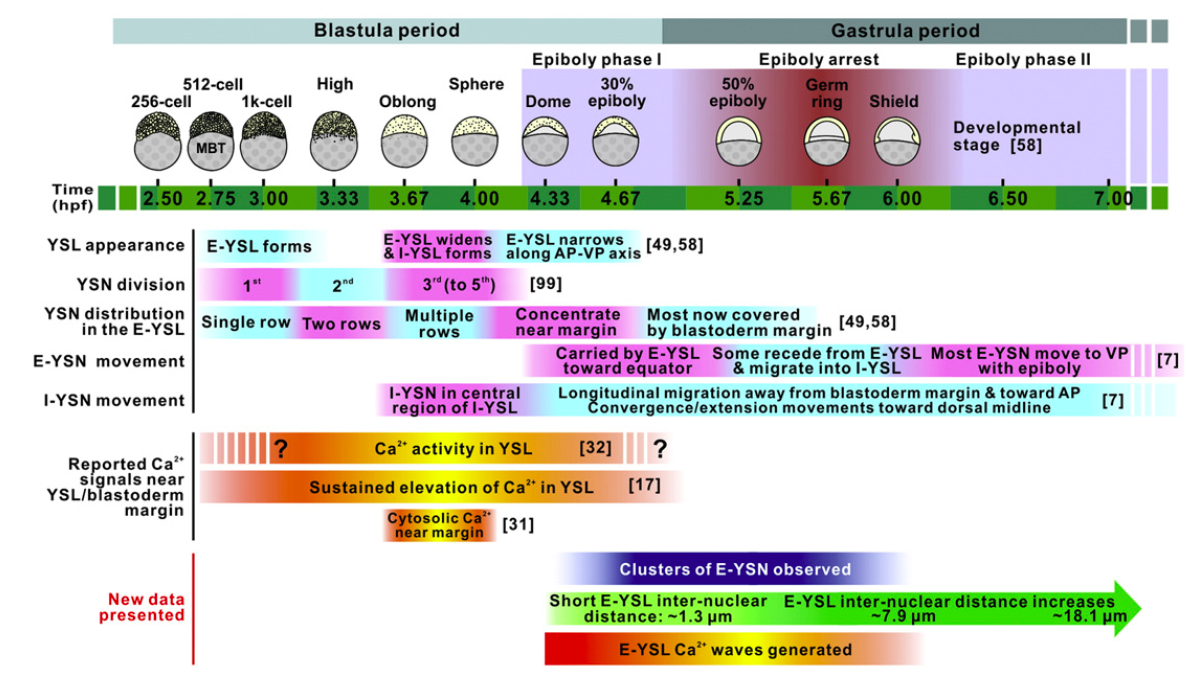
\includegraphics[width=0.8\textwidth]{../../images/zebrafish_10h_review/yuen_2012.png}
\end{center}
\caption{\textbf{Characterization of Ca(2+) signaling in the external yolk syncytial layer during the late blastula and early gastrula periods of zebrafish development. } Timeline to show the major events that occur during: the appearance of the YSL; the division, distribution and movement of the E-YSN; the movement of the I-YSN; and the reported Ca2+ signals generated at or near to the blastoderm margin, during the blastula and early gastrula periods. New data regarding E-YSN clustering, changes in inter-nuclear distance in the E-YSL over time and the generation of E-YSL Ca2+ waves are also shown. MBT, midblastula transition; AP, animal pole; VP, vegetal pole. These features correlating events at different scales does not bring us closer however to an integrated model of zebrafish blastulation and gastrulation. But it indeed provides some hints in the ingredients that the model should take into account. Figure and caption from Yuen et al., 2012 \cite{Yuen:2012fr}}
\label{zebrafish_10h_review_yuen_2012}
\end{figure}

EVL cells are obviously stretched, and as Rohde (2007) \cite{Rohde:2007ba} puts it: "It is possible this increase in surface area is not only a passive response to EVL stretching, but also an active component of epiboly. Experiments in \textit{Fundulus} showing an increase in apical membrane turnover in EVL cells under tension support this idea." This view is also supported by the work of Fink et al. \cite{Fink:1996un}.

As shown from lineage tracing experiments \cite{Kimmel:1985vc}, the progeny of injected deep cell starts to loose their cohesion during the 4th-hour period of development, indicating their newly acquired intrinsic motility \cite{Warga:1990vu}. From the sphere stage to the shield stage, the deep cells undergo radial intercalation. How much of this feature is the cause or consequence of this first phase of epiboly is unclear. Radial intercalation might indeed entrain the blastoderm margin and lead the epiboly movement of both the EVL and YSN. Deep cells might also actively migrate on the yolk and on the EVL to produce a similar phenotypic feature.

The role of the yolk in this first phase of epiboly might be envisioned at different levels. We already suggested a possible relative weakness of the yolk cortex that would contribute to the doming initiation. Then, although the literature does not mention this possibility, we might think about an active role of the yolk content, platelets and lipid drops, if moved by an internal cytoskeleton and molecular motors. To our knowledge, however, none of these are documented in the literature. Certain functions of the yolk cortical layer and its cytoskeleton are documented. Microtubules in the yolk cortical layer (iYSL) are absent in nocodazole treated embryos \cite{SolnicaKrezel:1994wl}. Consequently, the yolk cell acquires a more spherical shape and in addition, "the YSN are blocked in their movement towards the vegetal pole and do not exhibit elongated shapes. Deep cells move very slowly toward the vegetal pole and almost cover the YSN. Epiboly of the EVL is slower than in control embryos." However, epiboly is not impaired in nocodazole treated embryos and the process robustness indicates the synergistic involvement of multiple factors. Actomyosin contraction at the margin has been involved in the second phase of epiboly, although recent studies dispute its role \cite{Behrndt:2012gy}. Phase 1 epiboly would be however rather counteracted by a contraction at the blastoderm margin, with eventually the blastoderm slipping away from the yolk.
%  ====================================================================== 


\subsection{Gastrulation Movements}
%  ====================================================================== 


Gastrulation \textit{per se} starts by 6 hpf and is characterized by the involution of the endomesoderm most prominent on the dorsal side, the second phase of epiboly, and the beginning of convergence-extension movements. During gastrulation, it looks like blastoderm cells, YSN, and probably also the extra cellular matrix (ECM) have the same kind of movements. As a rough approximation, all cells and tissues move in a similar fashion. They spread over the yolk toward the vegetal pole (epiboly) and converge toward the dorsal side of the embryo to form the antero-posterior axis (convergence-extension).

However, the detailed observation of cells and tissues kinematics reveals that each tissue has specificities and their mechanical contribution to the gastrulation movements may be different. This issue is of importance to implement a relevant model of gastrulation processes.

Whether cells are active or passive, with homogenous behaviors within a tissue, exerting or not forces on neighboring tissues is difficult to assess. Perturbations, whether genetic, pharmacologic, or mechanic, have been extensively used to discriminate between different scenarios.
%  ---------------------------------------------------------------------- 


\subsubsection{Epiboly Phase Two}
%  ---------------------------------------------------------------------- 


Although epiboly might be considered a continuous process, it probably in fact relies on different processes distinguishing phase 1 and phase 2. Phase 2 epiboly coincides with the onset of gastrulation \textit{per se}. Again, gastrulation and epiboly seem robust to a number of perturbations and it seems possible to broadly decorrelate different processes contributing to normal gastrulation: epiboly, hypoblast formation/internalization, and convergence-extension.

What the driving force of epiboly is has not yet received a definitive answer. However, several hypotheses have been debated. The first explanation of epiboly in teleosts was proposed by J.P. Trinkaus in 1951 \cite{Trinkaus:1951ue}. He ruled out suppositions that epiboly was due to differential growth mechanisms or to a contractile activity of the yolk surface (the "yolk gel layer" idea). He rather favored the hypothesis that the so-called \textit{periblast} (now called the internal yolk syncytial layer iYSL) is responsible for the cells' \textit{mass movements}. This claim mainly relied on microdissection experiments in which the blastoderm was removed, leaving the periblast exposed. In such cases, the periblast still completed epiboly until the blastopore closure. Later studies \cite{Trinkaus:1967uz}\cite{Trinkaus:1984wu} confirmed this insight and designated the YSL as the driving force of Fundulus's epiboly. Despite a colchicine treatment of the Fundulus gastrulae, which blocked microtubule polymerization and impaired the deep cells' mechanical properties, the epiboly still performed normally \cite{Trinkaus:1983bm}. This led to the idea that deep cells are not responsible for the late epiboly: "Epiboly of Fundulus, and presumably of teleosts generally, does not depend on the deep cells." \cite{Trinkaus:1984wu}.

The possible scenarios differ in their explanation of the mechanisms underlying the vegetal-oriented displacement of the EVL, blastoderm and external YSL (eYSL) margin. In any case, it seems that a strong cohesion of the yolk membrane and EVL margin with the presence of tight junctions excludes the migration of EVL cells on the yolk membrane \cite{Betchaku:1978hm}. Other possible mechanisms include:
\begin{itemize}
	\item an autonomous YSL mechanism involving the microtubule network associated with the YSN
	\item endocytosis in the external YSL
	\item a passive EVL mechanism due to the internalizing treadmill movement (indirect influence of the deep cells)
	\item an active EVL cell mechanism which would increase its surface (active intercalation or active surface increase)
	\item an active contraction of the actomyosin ring-like structure in the eYSL margin
	\item a friction force induced by a retrograde flow in the eYSL.
\end{itemize}

\paragraph{Endocytosis in the external YSL}
%  ++++++++++++++++++++++++++++++++++++++++++++++++++++++++++++++++++++++ 


Endocytosis has been observed in Fundulus just below the advancing margin of the blastoderm \cite{Betchaku:1978hm}, thus in the eYSL only. In the zebrafish, the endocytotic process was observed even if in the absence of YSL microtubules \cite{SolnicaKrezel:1994wl}. It is however unlikely that they play an active role in the epiboly of the margin as the endocytic vesicles integrate the surface of the eYSL more vegetally and do not integrate the surface of the iYSL, thus not contributing to its expansion \cite{Betchaku:1986tw}.

\paragraph{Possible roles of the EVL in driving epiboly}
%  ++++++++++++++++++++++++++++++++++++++++++++++++++++++++++++++++++++++ 


The possibility that the EVL either migrates over the yolk surface, or rearranges, or contracts, and by doing so contributes in different ways to epiboly have been discussed. Filopodial activity has been observed on the apicolateral surfaces of the EVL cells at the EVL-eYSL interface. These microspike-like structures suggest that EVL may have an active behavior at the margin \cite{Zalik:1999tx}. Keller and Trinkaus observed cell rearrangements in the enveloping layer suggesting that the EVL may be an active component of epiboly \cite{Keller:1987va}. EVL cells however do not perform large-scale rearrangements during epiboly. In particular, nothing has been described so far as for the "rosette" scenario in \textit{Drosophila}\cite{Blankenship:2006jg}. We interpret that epithelia performing active rearrangements may have a 'lateral'-to-'apical-basal' length ratio much closer to 1 than is observed in the EVL. Finally, an actomyosin contraction in the YSL induces EVL cell shape changes \cite{Koppen:2006fy}, correlating with margin contraction. And the resulting constriction has long been postulated to be the driving force of epiboly.

\paragraph{The purse-string scenario, contraction at the margin of the eYSL and/or EVL margin}
%  ++++++++++++++++++++++++++++++++++++++++++++++++++++++++++++++++++++++ 


The presence of F-actin-based structures at the margin after 50 percent epiboly was described as the following by Cheng \cite{Cheng:2004ff}:
\begin{quotation}  They are composed of two ring-like F-actin structures that form at the deep cell and enveloping layer margins of the blastoderm and a punctate actin band that develops in the external yolk syncytial layer. Treatment with cytochalasin B or the calcium chelator dibromo-BAPTA results in the disruption of all three of these actin-based structures, leading to the slowing or immediate arrest of epiboly, respectively, followed by a failure of yolk cell occlusion and the eventual lysis of the embryo through the vegetal pole region.  
\end{quotation}

These observations suggested the role of a contractile ring in the occlusion of the vegetal portion of the yolk cell during the Phase 2 of epiboly. A hypothesis is that the Phase 2 epiboly is driven by an actomyosin contraction at the margin of the EVL. The local density of actin at the EVL margin correlates with its deformation. And the process involves actin and myosin 2 recruitment within the yolk cytoplasm, as observed in Drosophila for the dorsal closure \cite{Koppen:2006fy}. This scenario has been recently challenged and the state of the art in the domain now comes from the following works, described next.

\paragraph{A friction force induced by a retrograde flow in the eYSL}
%  ++++++++++++++++++++++++++++++++++++++++++++++++++++++++++++++++++++++ 


A recent study hypothesized the existence of an additional and previously undescribed force that would pull the EVL-yolk margin vegetally by a flow-friction mechanism \cite{Behrndt:2012gy}. This mechanism is shown to be sufficient to drive epithelial epiboly after 50 percent epiboly because, in mechanically constrained cylindrical embryos where a purse-string scenario is inefficient, the margin is still converging to the vegetal pole. We propose however that radial intercalation in the epiblast could explain the sustained epiboly in cylindrical embryos. This hypothesis might be tested by in vivo imaging and assess the position of the blastoderm margin compared to the EVL margin.

\paragraph{Blastoderm driving late epiboly}
%  ++++++++++++++++++++++++++++++++++++++++++++++++++++++++++++++++++++++ 
  XXXX pas encore OK chez nadine  
%  ====================================================================== 


\subsection{Convergence-Extension}
%  ====================================================================== 
  XXXX   
